% Untangling Federal Jurisdiction
% Part 1 of 3

% All content comes from Stephen Pratt. I have no idea if he approves of this effort or not.

\documentclass{beamer}
\usetheme{Madrid}
%\usetheme{Goettingen}
\usefonttheme{serif}
\usefonttheme{structuresmallcapsserif}
% \usepackage[font=small,labelfont=bf]{caption}
\usepackage{xcolor}
\usepackage{rotating}

\setbeamerfont{section title}{parent=title}
\setbeamercolor{section title}{parent=titlelike}
\defbeamertemplate*{section page}{default}[1][]
{
    \centering
    \begin{beamercolorbox}[sep=8pt,center,#1]{section title}
        \usebeamerfont{section title}\insertsection\par
    \end{beamercolorbox}
}
\newcommand*{\sectionpage}{\usebeamertemplate*{section page}}

\def\Put(#1,#2)#3{\leavevmode\makebox(0,0){\put(#1,#2){#3}}}

\makeatletter
\setbeamertemplate{footline}
{
    % Commented out to remove footer line entirely
%    \leavevmode%
%    \hbox{%
%    \begin{beamercolorbox}[wd=.333333\paperwidth,ht=2.25ex,dp=1ex,center]{author in head/foot}%
%        \usebeamerfont{author in head/foot}\insertshortauthor%~~\beamer@ifempty{\insertshortinstitute}{}{(\insertshortinstitute)}
%    \end{beamercolorbox}%
%    \begin{beamercolorbox}[wd=.333333\paperwidth,ht=2.25ex,dp=1ex,center]{title in head/foot}%
%        \usebeamerfont{title in head/foot}\insertshorttitle
%    \end{beamercolorbox}%
%    \begin{beamercolorbox}[wd=.333333\paperwidth,ht=2.25ex,dp=1ex,right]{date in head/foot}%
%        \usebeamerfont{date in head/foot}\insertshortdate{}\hspace*{2em}
%        \insertframenumber{} / \inserttotalframenumber\hspace*{2ex} 
%    \end{beamercolorbox}}%
%    \vskip0pt%
}
\makeatother

\newenvironment<>{varblock}[2][\textwidth]{
    \begin{center}
        \begin{minipage}{#1}
            \setlength{\textwidth}{#1}
            \begin{actionenv}#3
                \def\insertblocktitle{#2}
                \par
                \usebeamertemplate{block begin}}
            {\par
                \usebeamertemplate{block end}
            \end{actionenv}
        \end{minipage}
    \end{center}
}

\DeclareGraphicsExtensions{.pdf,.png,.jpg}


\usepackage[utf8]{inputenc}
\def\braces#1{[#1]}
\begin{document}

\title[Untangling Federal Jurisdiction]{Untangling Federal Jurisdiction Within a State}
\author{Stephen Pratt}

\section{A Recurrence to First Principles}

\myquote{Benjamin Franklin}{img/ben-franklin.png}{``A frequent recurrence to \emph{fundamental principles}\ldots is absolutely necessary to preserve the blessings of liberty and keep a government free.''}

\myquote{Patrick Henry}{img/patrick-henry.png}{%
``No free government, or the blessing of liberty, can be preserved to any people but\ldots by a frequent recurrence to \emph{fundamental principles}}

\myquote{Supreme Court, Fletcher vs. Peck, Supreme Court, 1810}{img/supreme-court-1810.png}{%
``The security of a people against the misconduct of their rulers,
must lie in the frequent recurrence to \emph{first principles}, and
the imposition of adequate constitutional restrictions.''}

\myquote{Winston Churchill, ``Statehood'', p. 19}{img/winston-churchill-quotepage.png}{%
    ``The further back you can look, the farther forward you are likely to see.''%
}

\begin{frame}{Two Contending Forces}
    \begin{columns}[onlytextwidth]
        \column{0.5\textwidth}
            \centering
            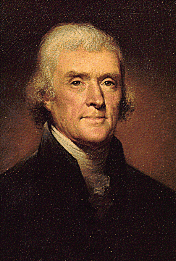
\includegraphics[height=0.75\textheight]{img/jefferson.png} \\
            Thomas Jefferson, 1824

        \column{0.5\textwidth}
            Men by their constitutions are naturally divided into two parties: \\
            \begin{enumerate}
                \item Those who fear and distrust the people, and wish to draw all powers from them into the hands of the higher classes.
                \item Those who identify themselves with the people, [and] have confidence in them.
            \end{enumerate}
    \end{columns}
\end{frame}

\begin{frame}{Theban Legion}
    \centering
    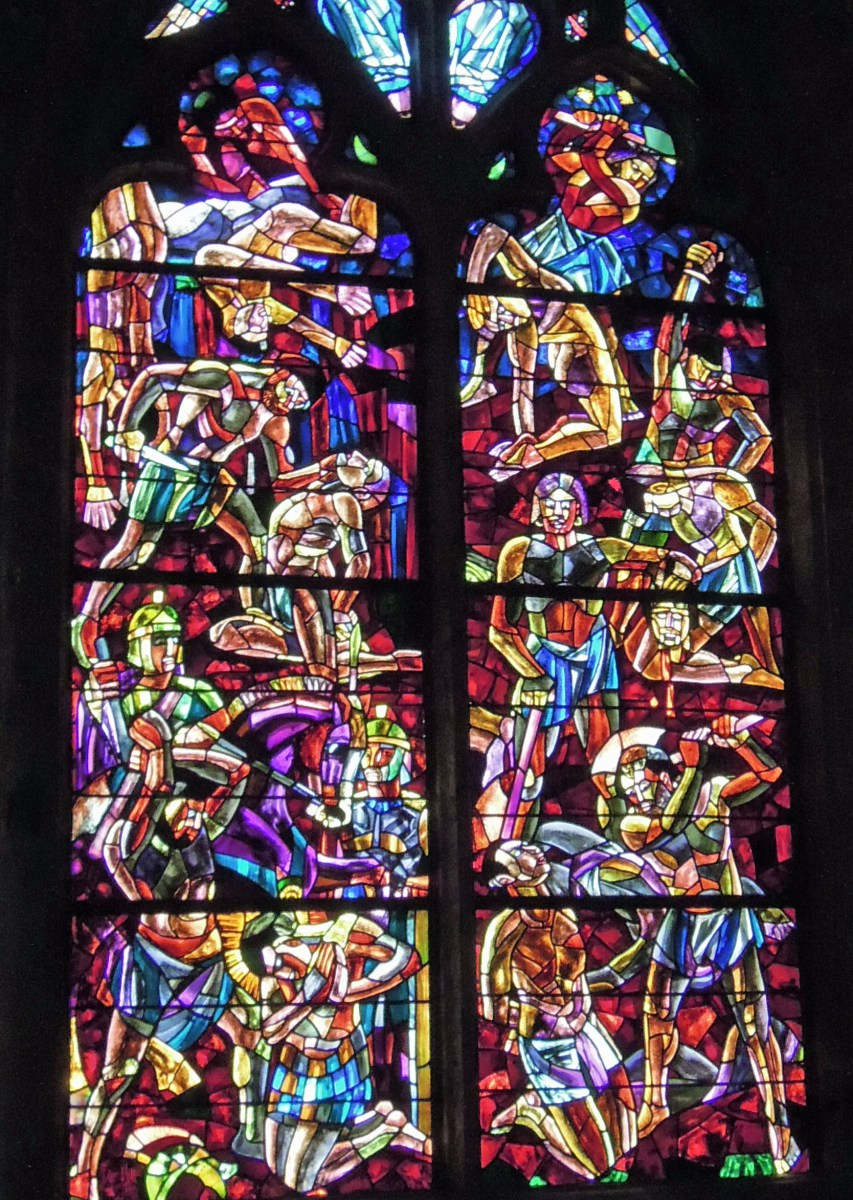
\includegraphics[height=0.7\textheight]{img/theban-1.jpg} \\
    Abbaye de Saint-Maurice, Switzerland. Stained glass by Swiss artist Edmond Bille. \\
\end{frame}

\begin{frame}{The World's Plan for Happiness}
    \centering
    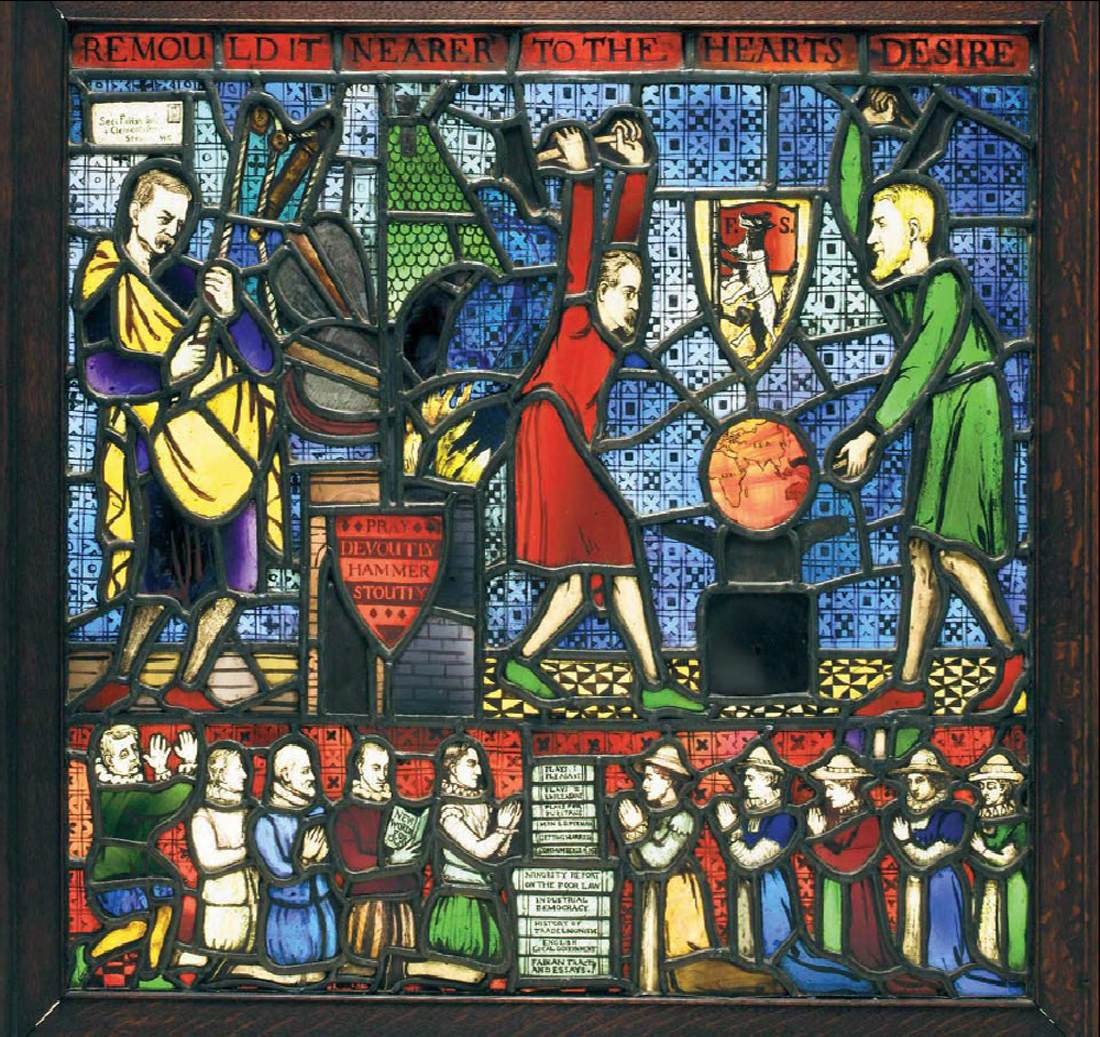
\includegraphics[height=.9\textheight]{img/remold-it.jpg} \\
\end{frame}

%\begin{frame}{Theban Legion}
%    \centering
%    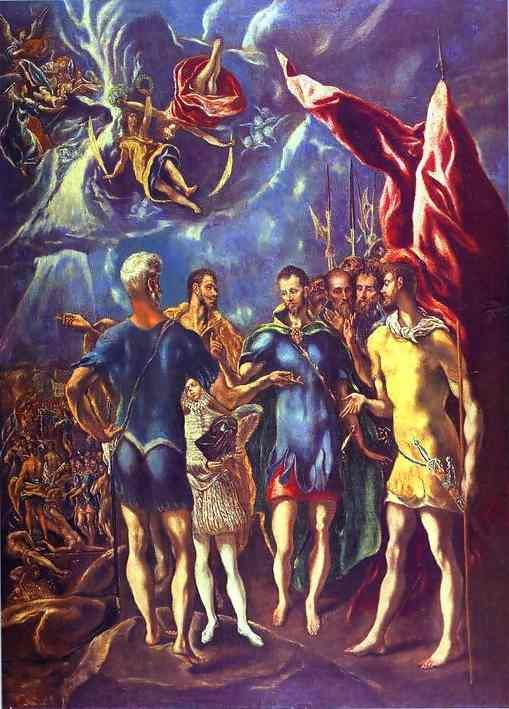
\includegraphics[height=0.8\textheight]{img/theban-2.jpg} \\
%    ``The Martyrdom of Maurice and the Theban Legion'', El Greco, ca. 1580  \\
%\end{frame}

\begin{frame}{Theban Legion}
    \centering
    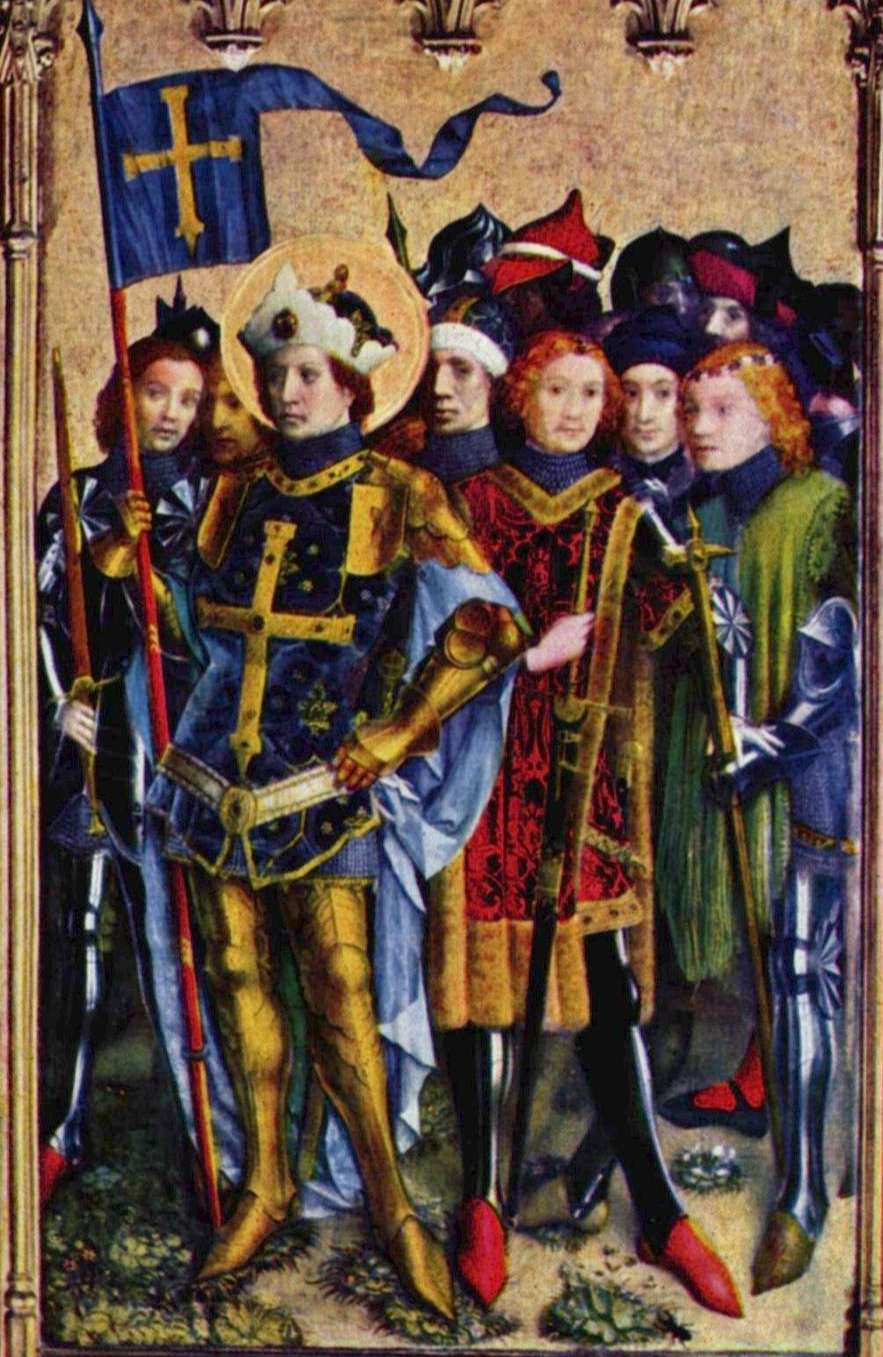
\includegraphics[height=0.7\textheight]{img/theban-3-clip.png} \\
    ``Saint Gereon of the Theban Legion and soldier companions'', Stefan Lochner, ca. 1440 \\
\end{frame}

%\begin{frame}{Theban Legion}
%    \centering
%    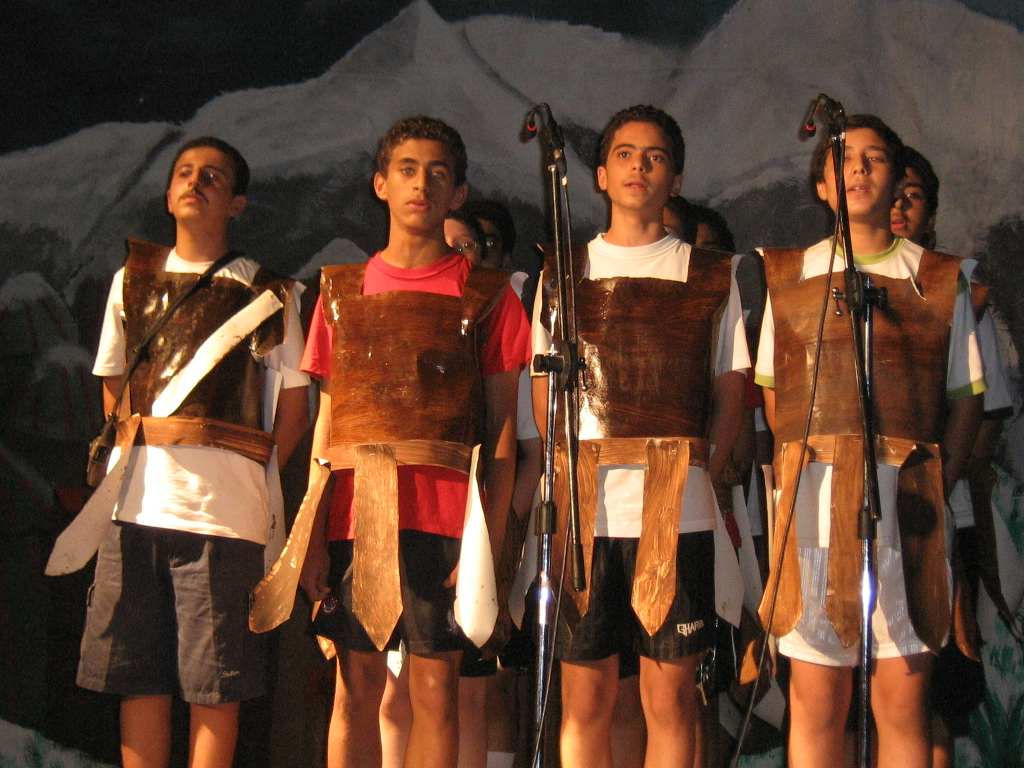
\includegraphics[height=0.8\textheight]{img/theban-4.jpg} \\
%    The Theban Legion probably didn't look much like this. \\
%\end{frame}

%\begin{frame}{Roman Civil Law, 9 A. D.}
%    \centering
%    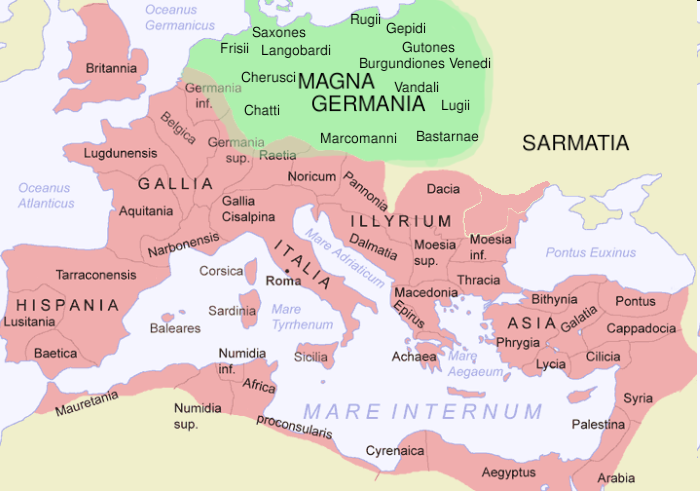
\includegraphics[width=0.75\textwidth]{img/europe-map.png} \\
%    \only<1>{Roman Law \\}
%%    \only<2>{Civil Law \\}
%%    \only<3>{Roman Civil Law \\}
%\end{frame}
%
%\begin{frame}{Roman Law}
%    \begin{columns}[onlytextwidth]
%        \column{0.5\textwidth}
%            \centering
%            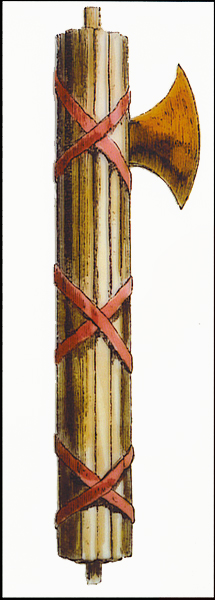
\includegraphics[height=0.55\textheight]{img/fasces-copy.jpg} \\
%            Fasces \\
%
%        \column{0.5\textwidth}
%            \begin{itemize}
%                \item All powerful central government
%                \item National sovereignty
%                \item Tax and control everything
%                \item Watchdog everyone's business
%                \item Promise prosperity and greatness
%                \item Fight wars anywhere on earth
%                \pause
%                \item \emph{Do whatever is necessary. No exceptions. No limits\ldots}
%            \end{itemize}
%    \end{columns}
%\end{frame}
%
%\begin{frame}
%    \centering
%    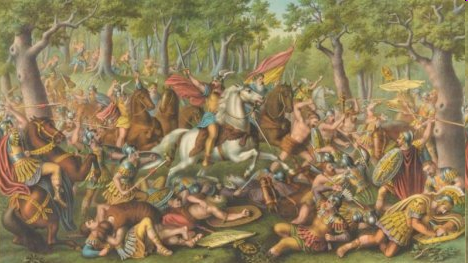
\includegraphics[width=0.95\textwidth]{img/teutoburg.png} \\
%    Battle of Teutoburg Forest, 9 A. D. \\
%        Arminius of the Cherusci, Publius Quinctilius Varus \\
%%    \only<2>{``We will rule our own territory!'' \\ }
%\end{frame}
%
%\begin{frame}
%    \centering
%    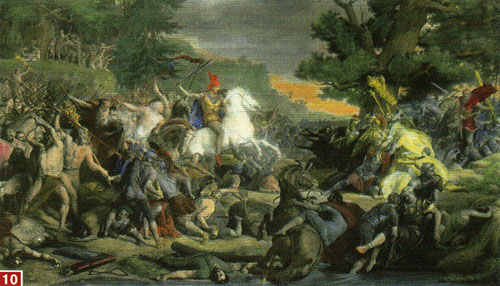
\includegraphics[width=0.95\textwidth]{img/teutoberg.jpg} \\
%    Battle of Teutoburg Forest, 9 A. D. \\
%        Arminius of the Cherusci, Publius Quinctilius Varus \\
%%    \only<2>{``We will rule our own territory!'' \\ }
%\end{frame}
%
%\begin{frame}
%    \centering
%    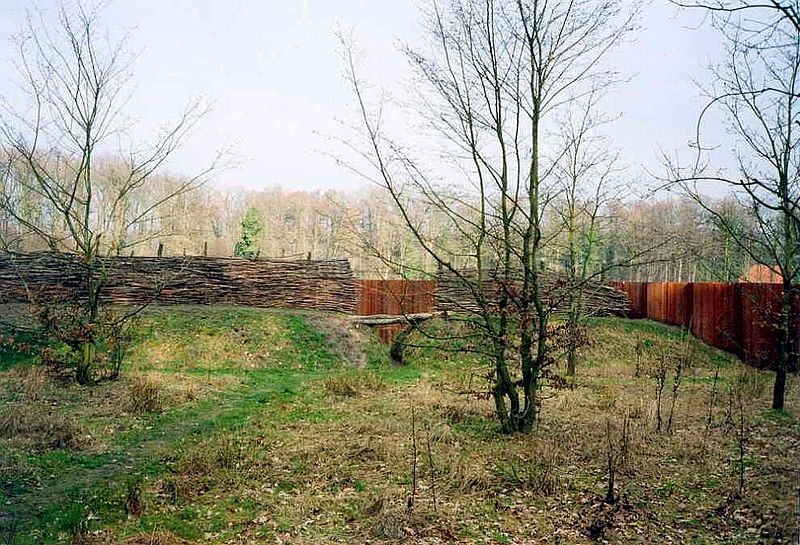
\includegraphics[width=0.95\textwidth]{img/Varus01.jpg} \\
%    Battle of Teutoburg Forest, 9 A. D. \\
%        Arminius of the Cherusci, Publius Quinctilius Varus \\
%%    \only<2>{``We will rule our own territory!'' \\ }
%\end{frame}
%
%\begin{frame}
%    \centering
%    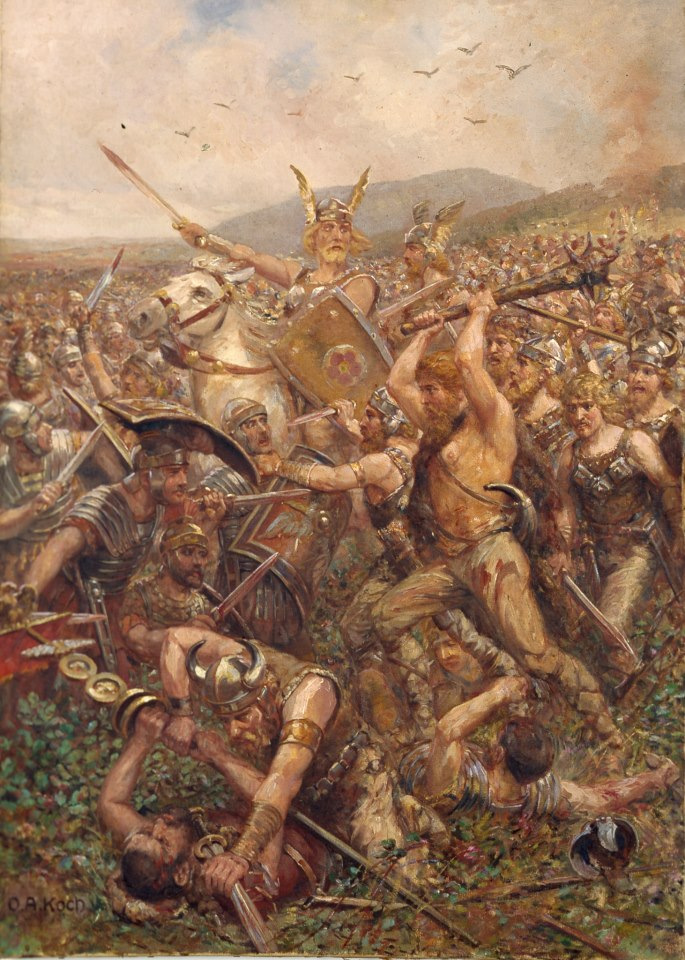
\includegraphics[height=0.8\textheight]{img/teut2.jpg} \\
%    Battle of Teutoburg Forest, 9 A. D. \\
%        Arminius of the Cherusci, Publius Quinctilius Varus \\
%%    \only<2>{``We will rule our own territory!'' \\ }
%\end{frame}
%
%\begin{frame}
%    \centering
%    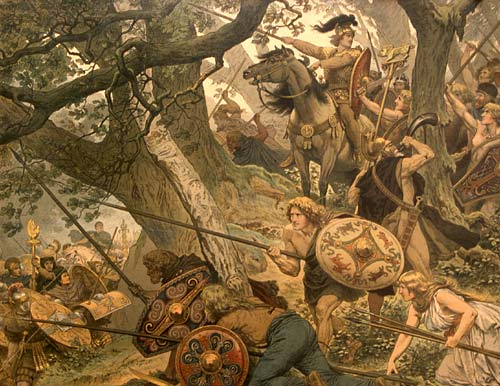
\includegraphics[height=0.8\textheight]{img/teut3.jpg} \\
%    Battle of Teutoburg Forest, 9 A. D. \\
%        Arminius of the Cherusci, Publius Quinctilius Varus \\
%%    \only<2>{``We will rule our own territory!'' \\ }
%\end{frame}
%
%\begin{frame}
%    \centering
%    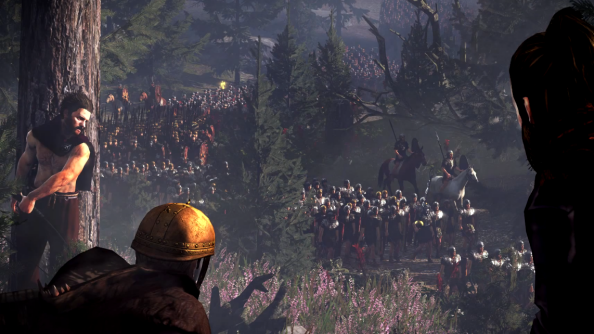
\includegraphics[width=0.95\textwidth]{img/teut4.png} \\
%    Battle of Teutoburg Forest, 9 A. D. \\
%        Arminius of the Cherusci, Publius Quinctilius Varus \\
%%    \only<2>{``We will rule our own territory!'' \\ }
%\end{frame}
%
%\begin{frame}
%    \centering
%    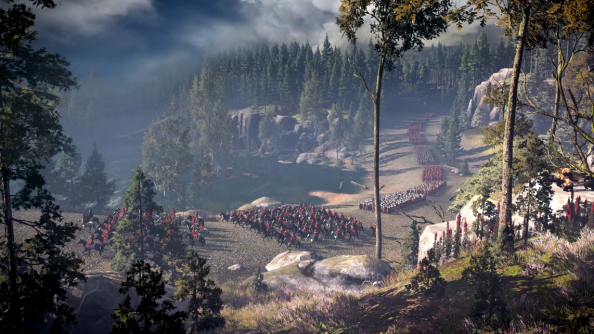
\includegraphics[width=0.95\textwidth]{img/teut5.png} \\
%    Battle of Teutoburg Forest, 9 A. D. \\
%        Arminius of the Cherusci, Publius Quinctilius Varus \\
%%    \only<2>{``We will rule our own territory!'' \\ }
%\end{frame}
%
%\begin{frame}{Anglo-Saxon Common Law}
%    \begin{columns}[onlytextwidth]
%        \column{0.5\textwidth}
%            Germanic brothers who entered England in 450 A. D., bringing with them Anglo-Saxon Common Law, the ``Guardian of Freedom''.
%
%        \column{0.5\textwidth}
%            \centering
%            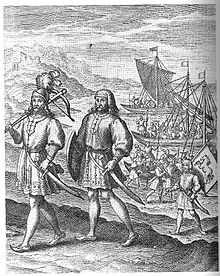
\includegraphics[height=0.55\textheight]{img/hengist-horsa.png} \\
%            Hengist and Horsa \\
%    \end{columns}
%\end{frame}

\begin{frame}{Germany, 1875 --- Hermanns Denkmal}
    \centering
    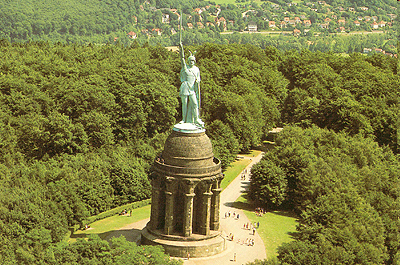
\includegraphics[width=0.75\textwidth]{img/hermans-denkmal.png} \\
\end{frame}

\begin{frame}{Germany, 1875 --- Hermanns Denkmal}
    \centering
    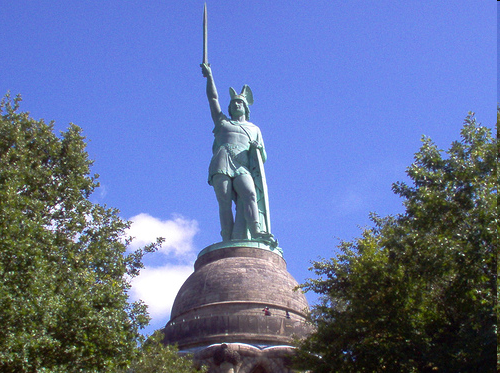
\includegraphics[width=0.75\textwidth]{img/herman2.png} \\
\end{frame}

%\begin{frame}
%    \begin{columns}[onlytextwidth]
%        \column{0.5\textwidth}
%            \centering
%            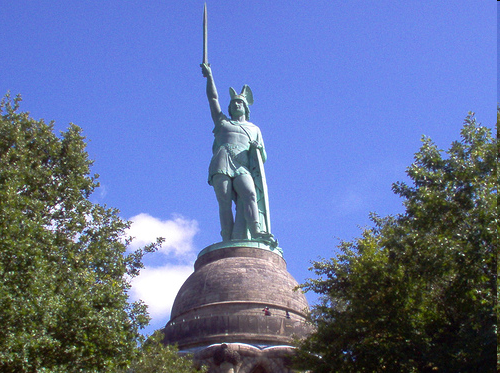
\includegraphics[width=0.75\textwidth]{img/herman2.png} \\
%
%        \column{0.5\textwidth}
%            Arminius / Herman preserved ``Common Law''
%            \pause
%            \begin{itemize}
%                \item Higher Law
%                \pause
%                \item Law of Nature
%                \pause
%                \item Constrast with Roman Law, based on coercion and force
%            \end{itemize}
%    \end{columns}
%\end{frame}
%
%\begin{frame}{Fundamental Principles of Common Law}
%    \centering
%    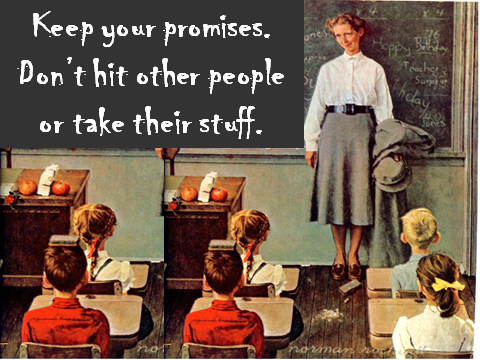
\includegraphics[width=0.75\textwidth]{img/schoolroom.png} \\
%\end{frame}
%
%\begin{frame}{Preserve Our Principles}
%    \centering
%    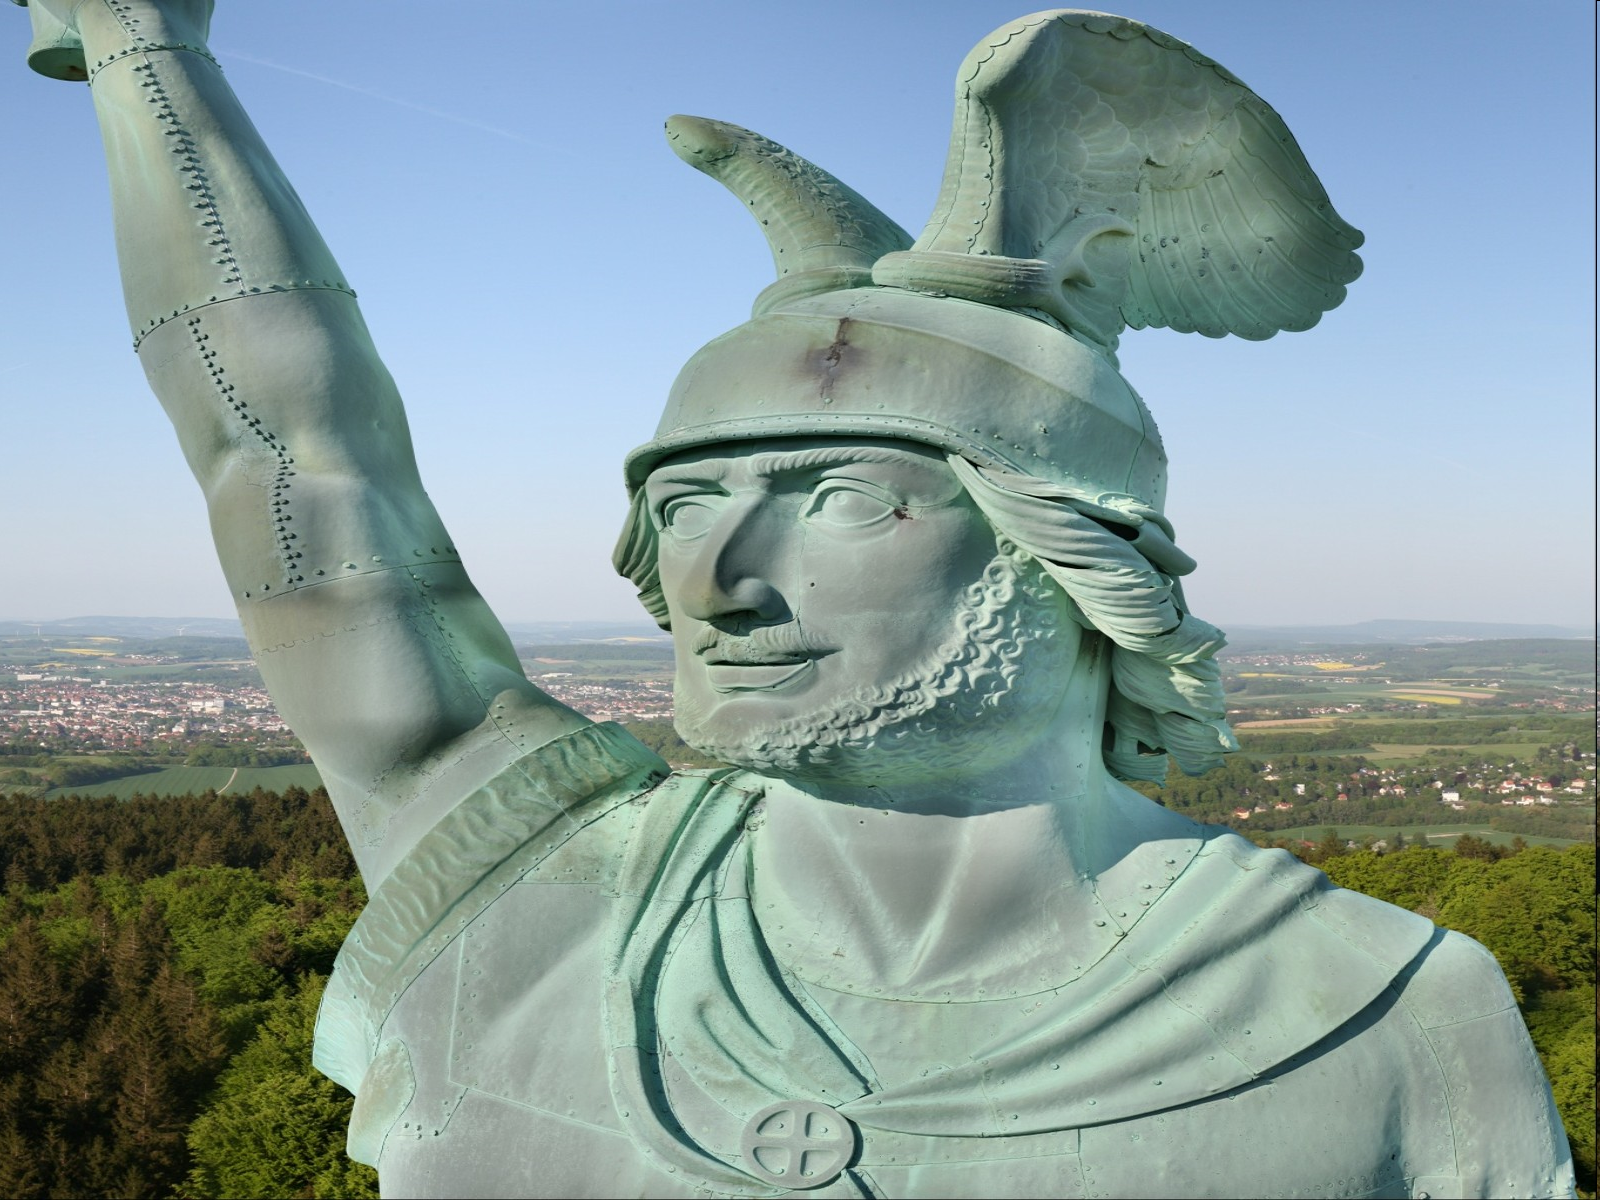
\includegraphics[width=0.75\textwidth]{img/herman3.png} \\
%    Rome, go home! \\
%\end{frame}
%
%\begin{frame}{Preserve Our Principles}
%    \begin{columns}[onlytextwidth]
%        \column{0.5\textwidth}
%            \centering
%            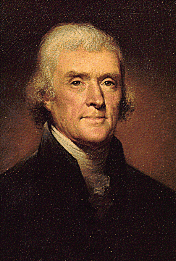
\includegraphics[width=0.75\textwidth]{img/jefferson.png} \\
%            Thomas Jefferson \\
%
%        \column{0.5\textwidth}
%            Restore the Ancient Principles\ldots
%            \begin{itemize}
%                \item \ldots of Common Law
%                \item \ldots of the Old Testament
%            \end{itemize}
%    \end{columns}
%\end{frame}

\begin{frame}{Government of Ancient Israel}
    \centering
    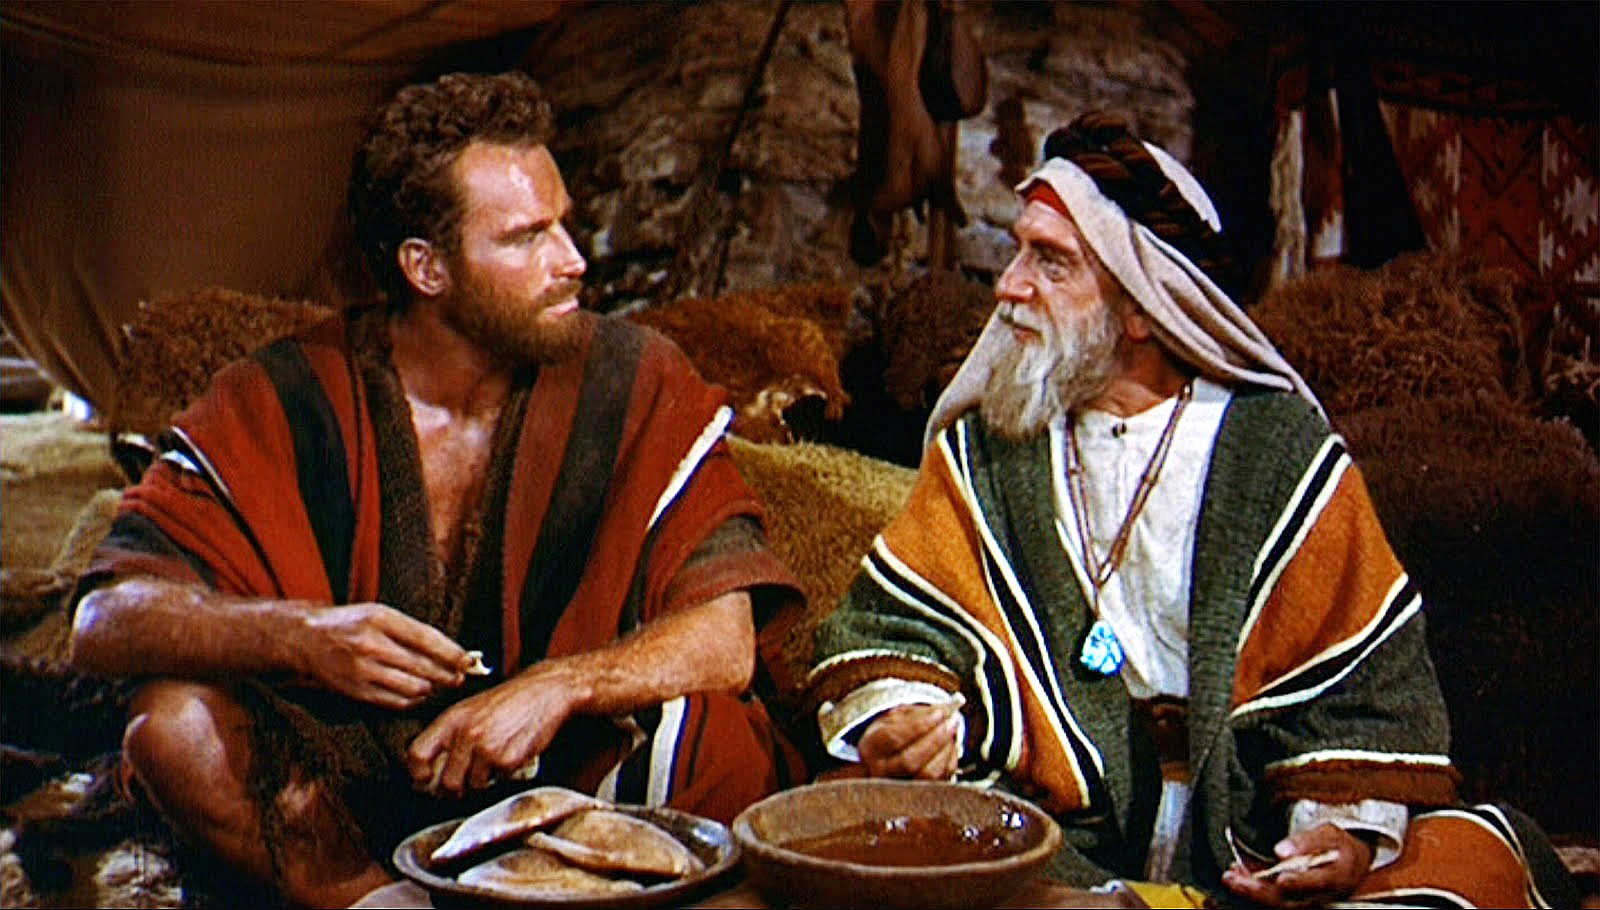
\includegraphics[width=0.75\textwidth]{img/moses.jpg} \\
    \only<1>{
        And Moses' father-in-law said unto him: Thou shalt teach them ordinances and laws, and shalt show them the way wherein they must walk and the work that they must do.
    }
    \only<2>{ Groups of tens, fifties, hundreds, thousands, to successfully govern three million people \\ }
%    \only<3>{ This became the basis of ``Common'', or ``People's'' Law \\ }
\end{frame}

%\begin{frame}{Preserve Our Principles}
%    \begin{columns}[onlytextwidth]
%        \column{0.5\textwidth}
%            \centering
%            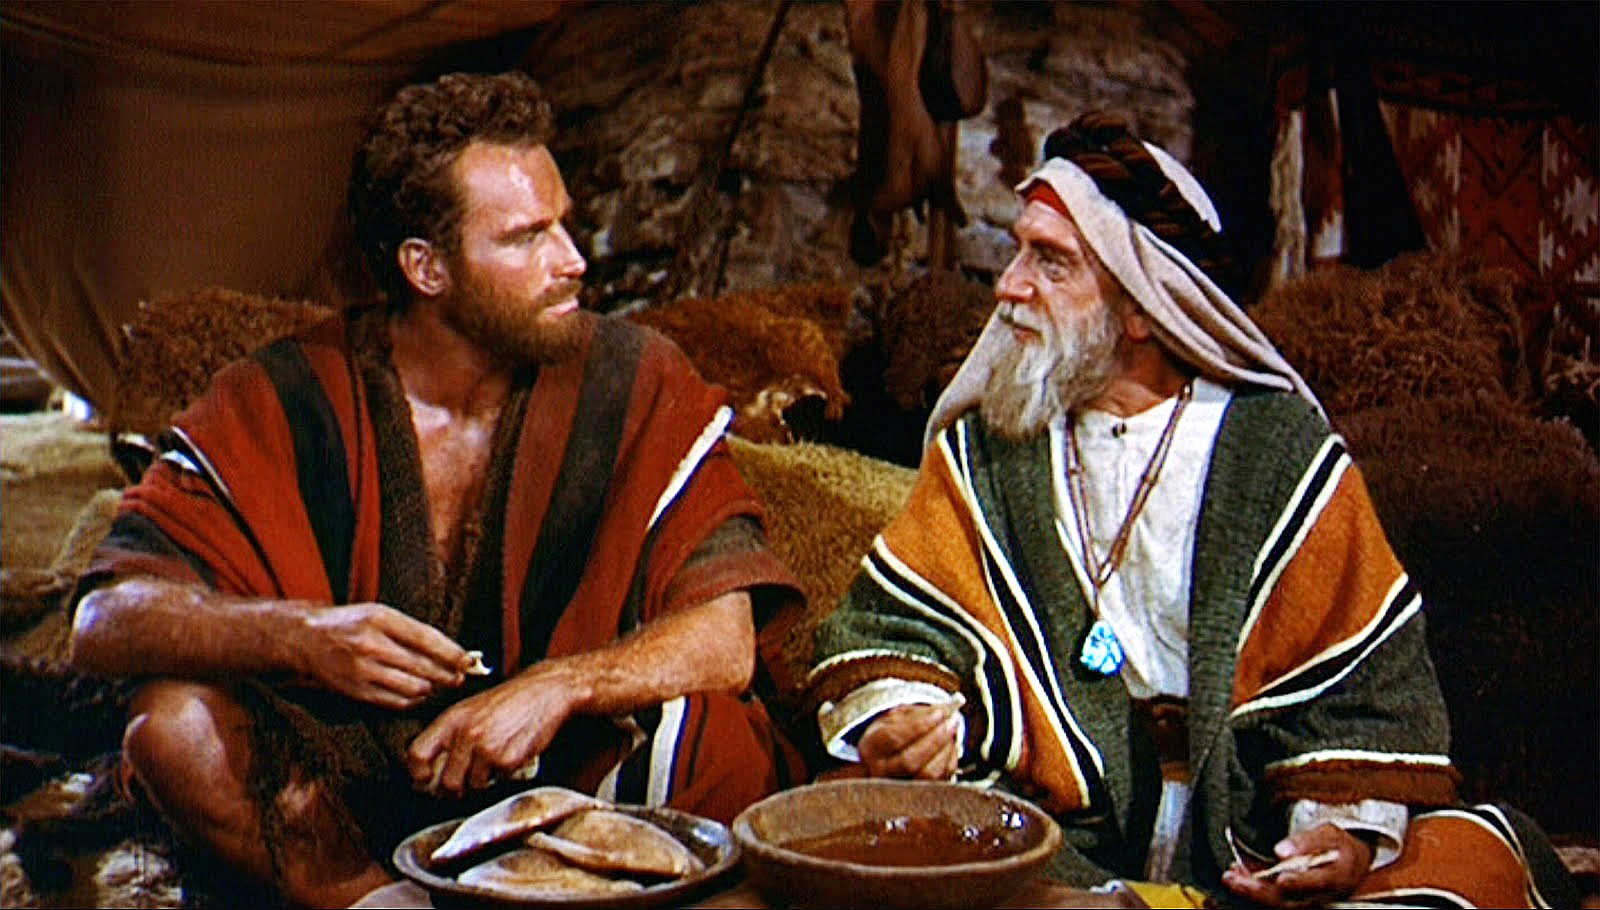
\includegraphics[width=0.75\textwidth]{img/moses.jpg} \\
%            Anglo-Saxon Common Law \color{red}\\
%
%        \column{0.5\textwidth}
%            \begin{itemize}
%                \item Ten families --- a ``Tithing'', led by a ``tithing man''
%                \item Two tithings --- a ``Vil'', led by a ``vil man''
%                \item Two vils --- a ``Hundred'', led by a ``hundred man''
%                \item Several hundreds --- a ``Shire'', led by a ``shire reef''
%            \end{itemize}
%    \end{columns}
%\end{frame}
%
%\begin{frame}{Roman Law v. Common Law}
%    \begin{columns}[onlytextwidth]
%        \column{0.5\textwidth}
%            \centering
%            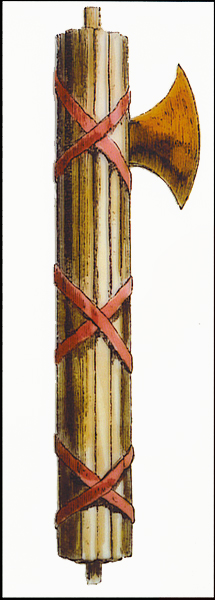
\includegraphics[height=0.75\textheight]{img/fasces-copy.jpg} \\
%
%        \column{0.5\textwidth}
%            \centering
%            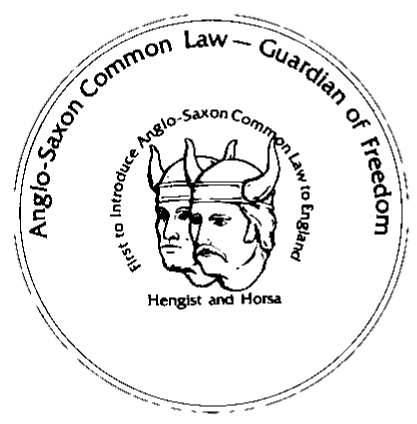
\includegraphics[height=0.35\textheight]{img/hh-coin.png} \\
%            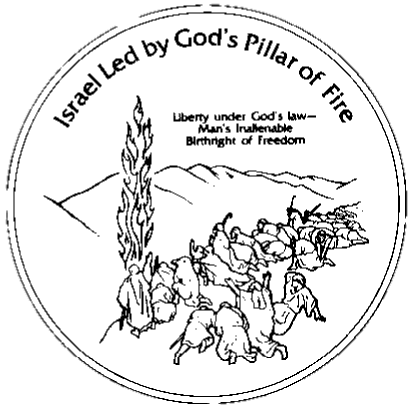
\includegraphics[height=0.35\textheight]{img/israel-coin.png} \\
%    \end{columns}
%\end{frame}

\begin{frame}{1914}
    \centering
    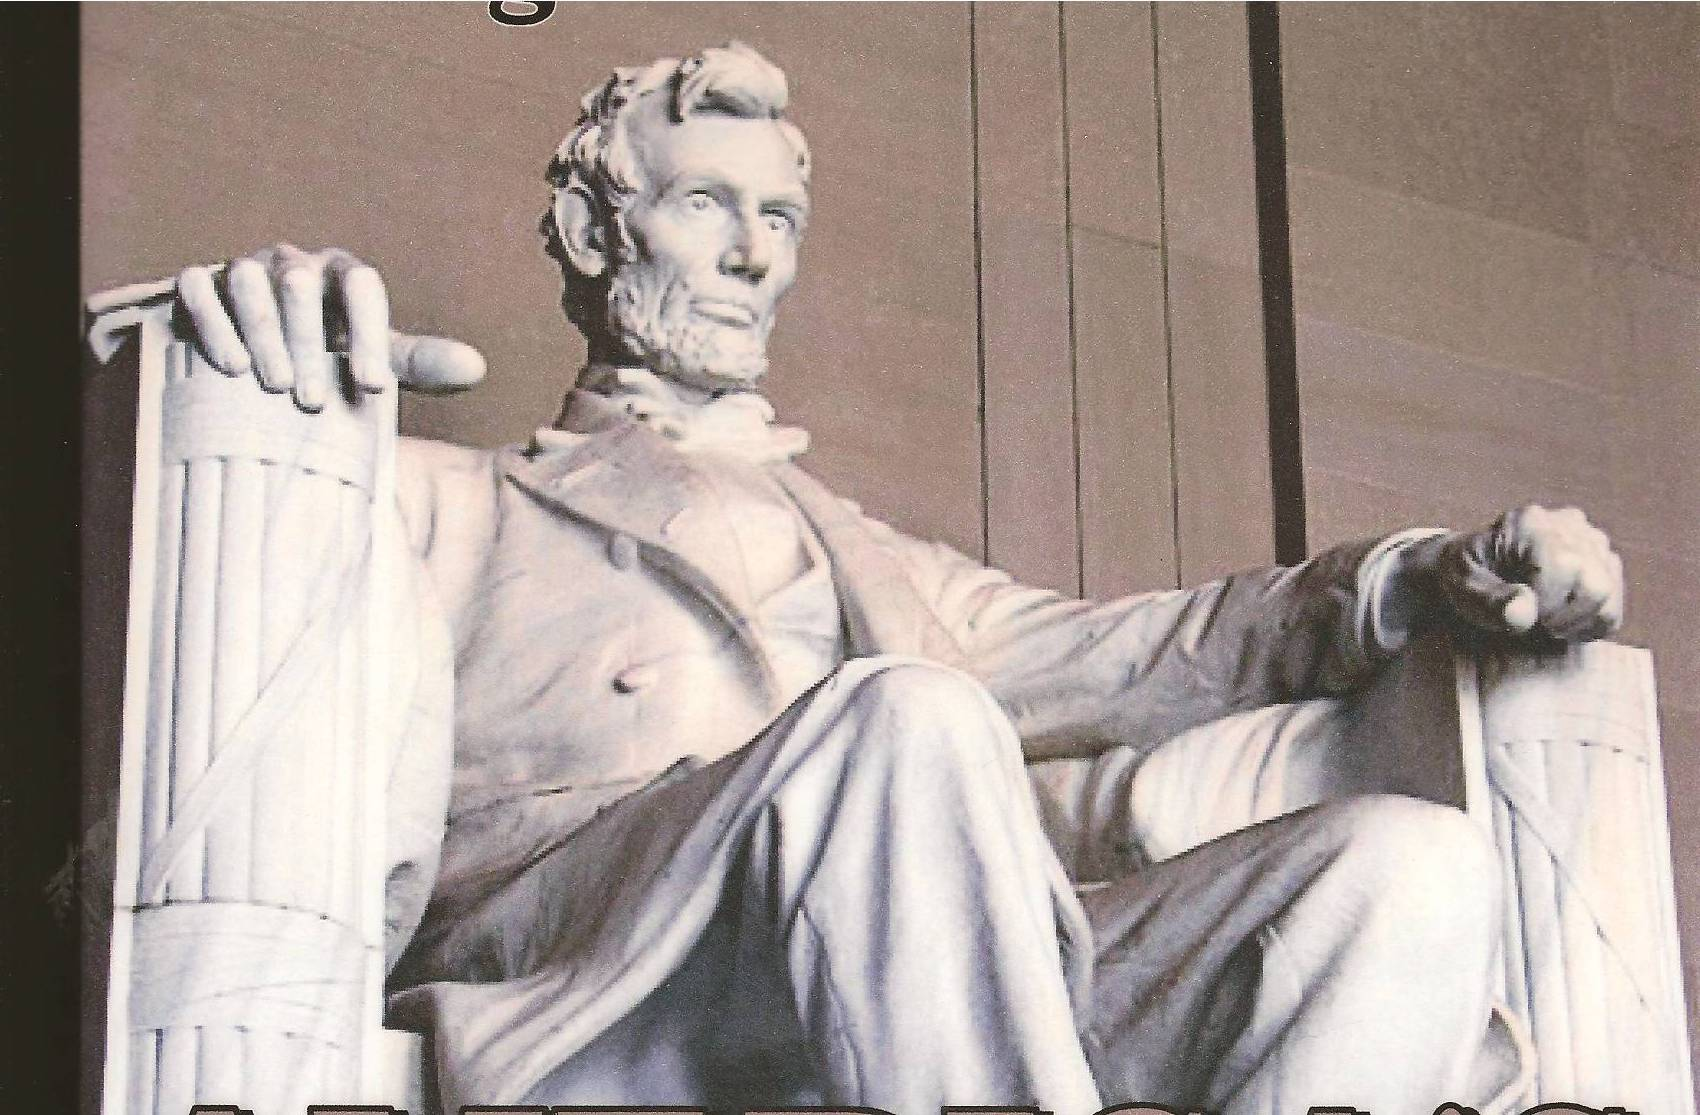
\includegraphics[width=.9\textwidth]{img/lincoln-memorial.jpg} \\
\end{frame}

\begin{frame}
    \begin{columns}[onlytextwidth]
        \column{0.5\textwidth}
            \centering
            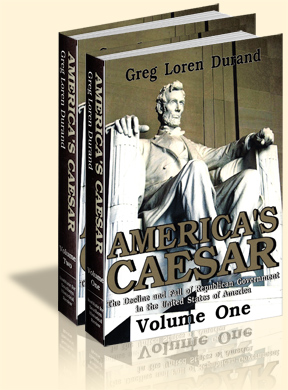
\includegraphics[width=0.75\textwidth]{img/americas-caesar.png} \\

        \column{0.5\textwidth}
            \begin{block}{America's Caesar}
                The Decline and Fall of Republican Government in the United States of America
            \end{block}
    \end{columns}
\end{frame}

\begin{frame}
    \begin{columns}[onlytextwidth]
        \column{0.5\textwidth}
            \centering
            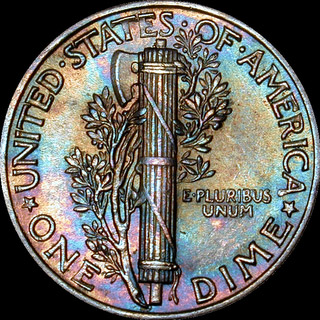
\includegraphics[width=0.75\textwidth]{img/dime-usa-fasces-2.jpg} \\
            1916 - 1945 \\

        \column{0.5\textwidth}
            \centering
            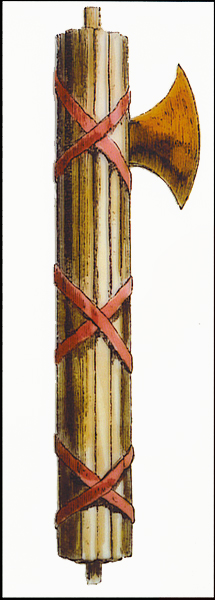
\includegraphics[height=0.55\textheight]{img/fasces-copy.jpg} \\
            Roman Law\\

    \end{columns}
\end{frame}

\begin{frame}
    \centering
    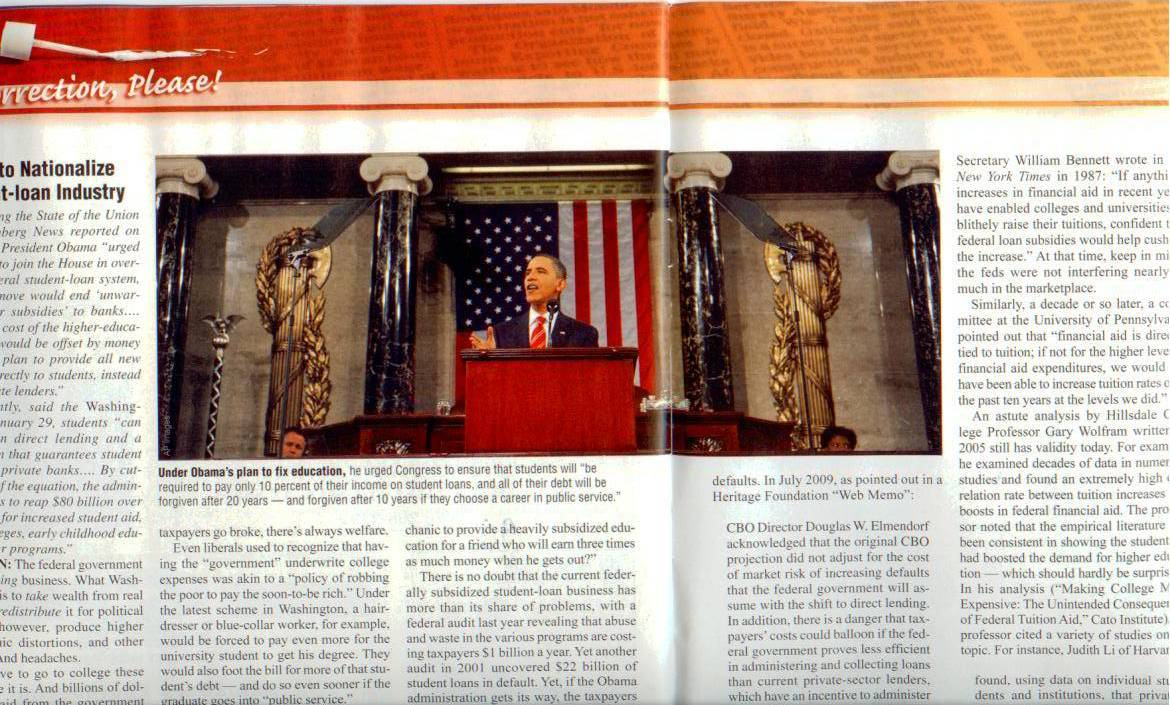
\includegraphics[width=.9\textwidth]{img/obama-fasces.jpg} \\
\end{frame}

\begin{frame}
    \centering
    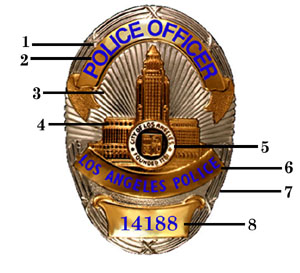
\includegraphics[height=.8\textheight]{img/fasces/badge_description.jpg} \\
    Los Angeles Police Dept. badge, developed 1939 - 1941 \\
\end{frame}
\begin{frame}
    \centering
    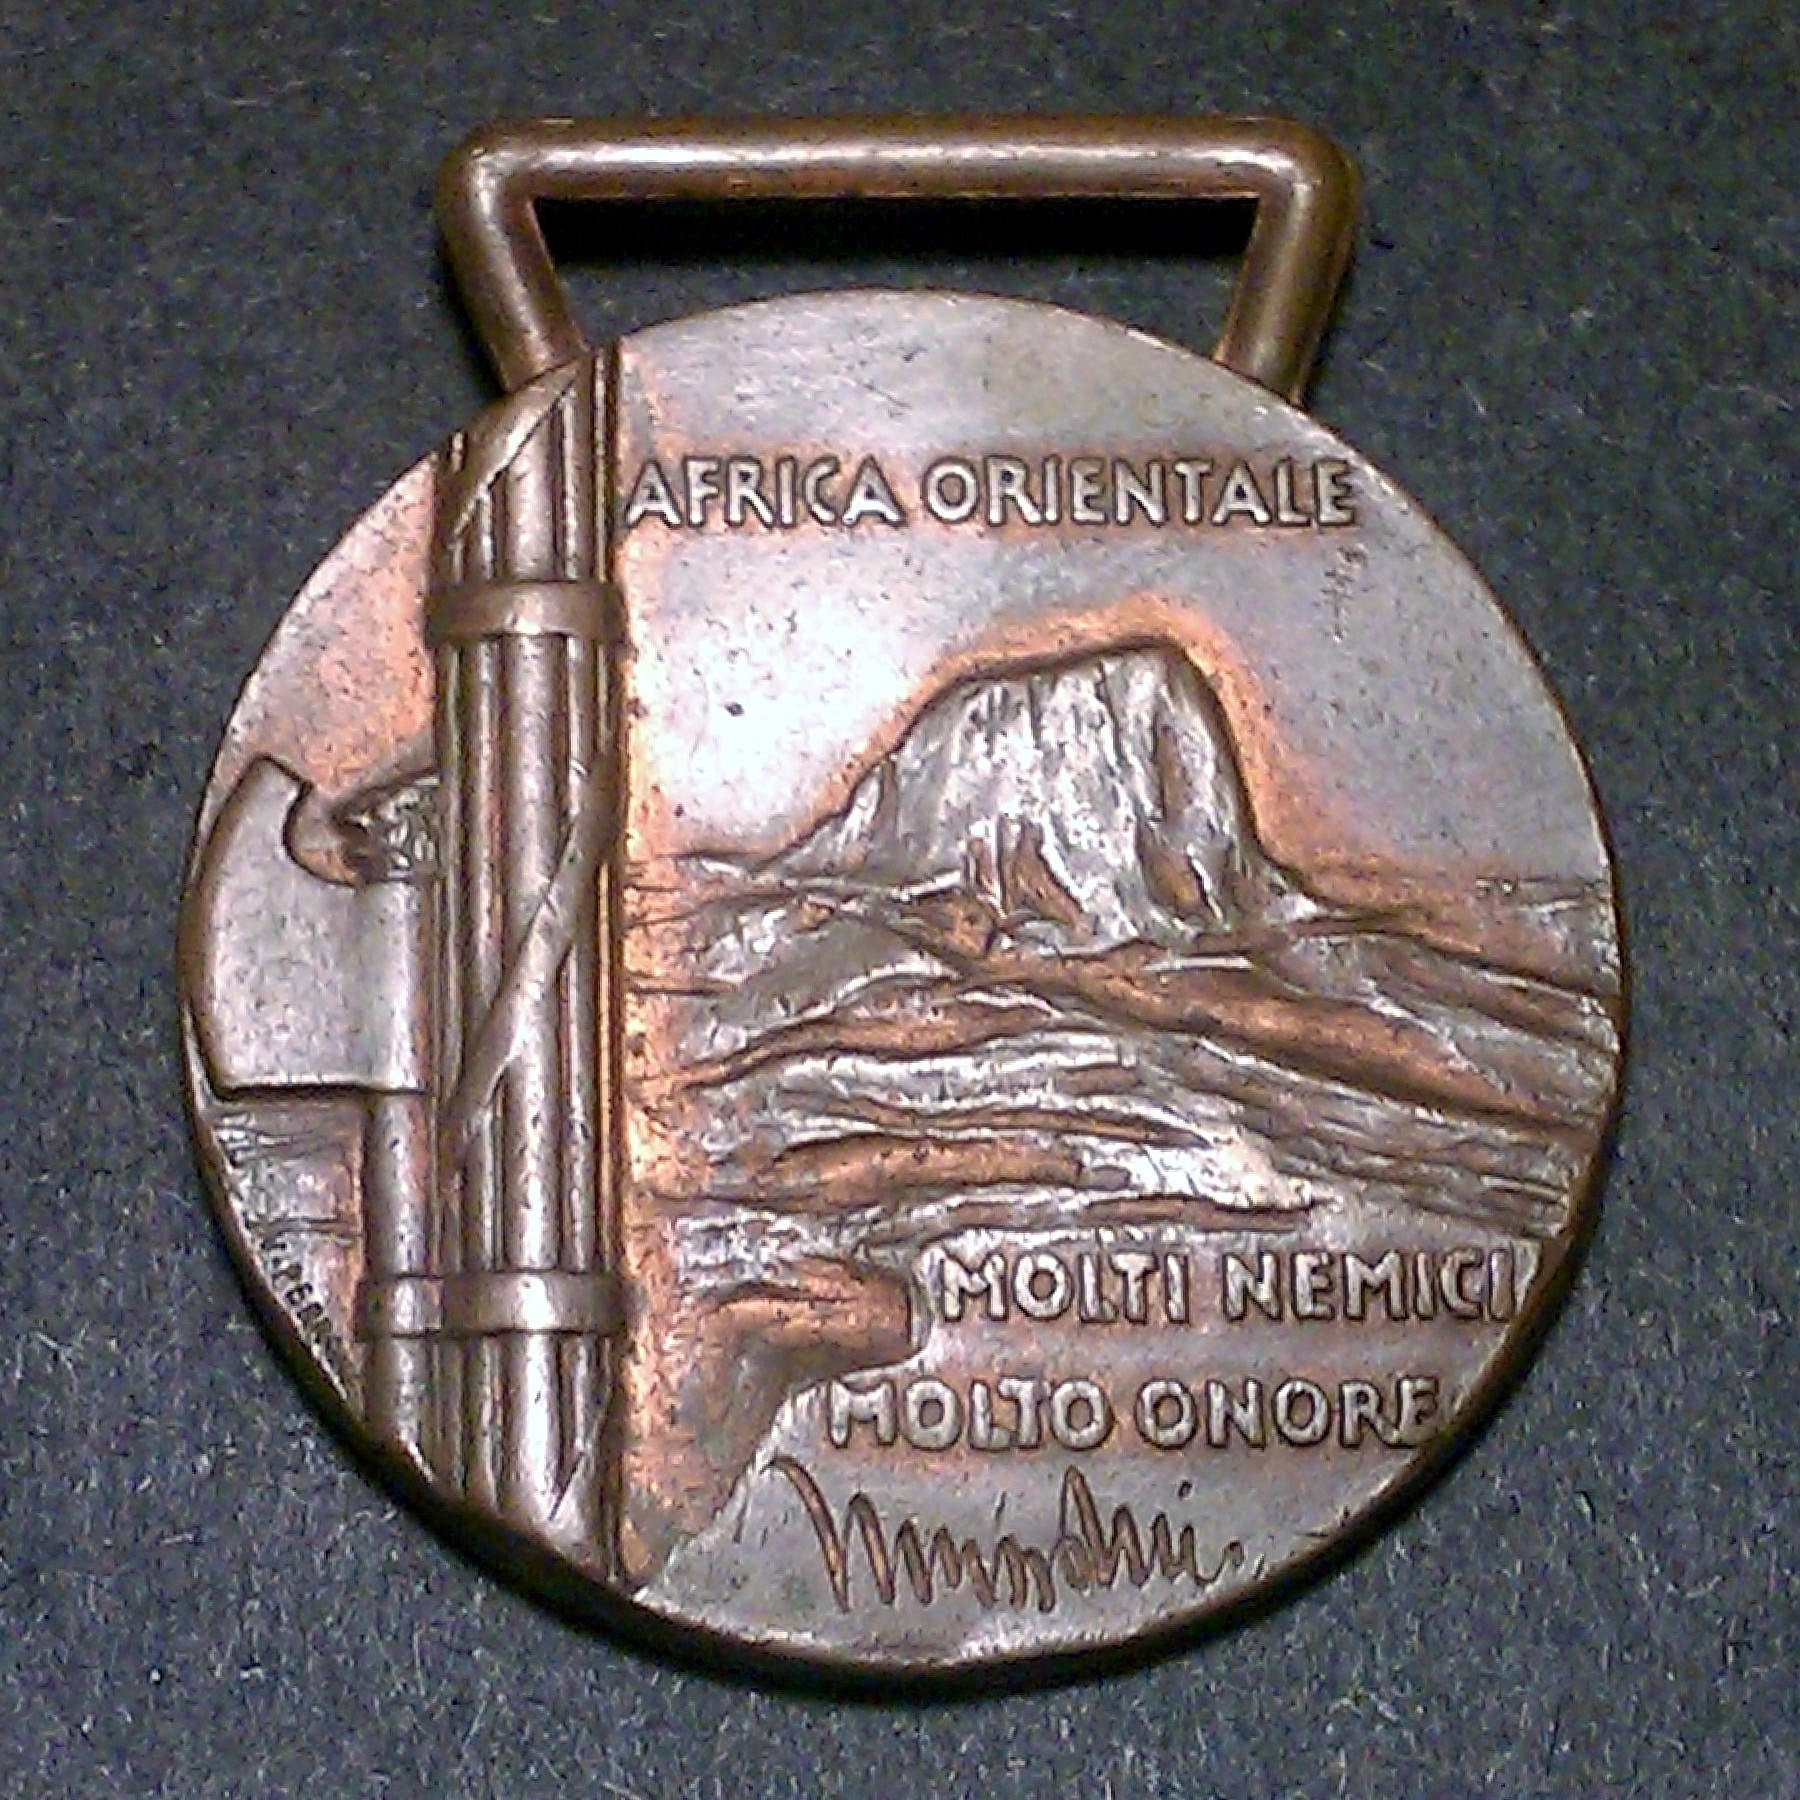
\includegraphics[height=.8\textheight]{img/fasces/coin.jpg} \\
    Italian East Africa Campaign medal, 1936 \\
\end{frame}
\begin{frame}
    \centering
    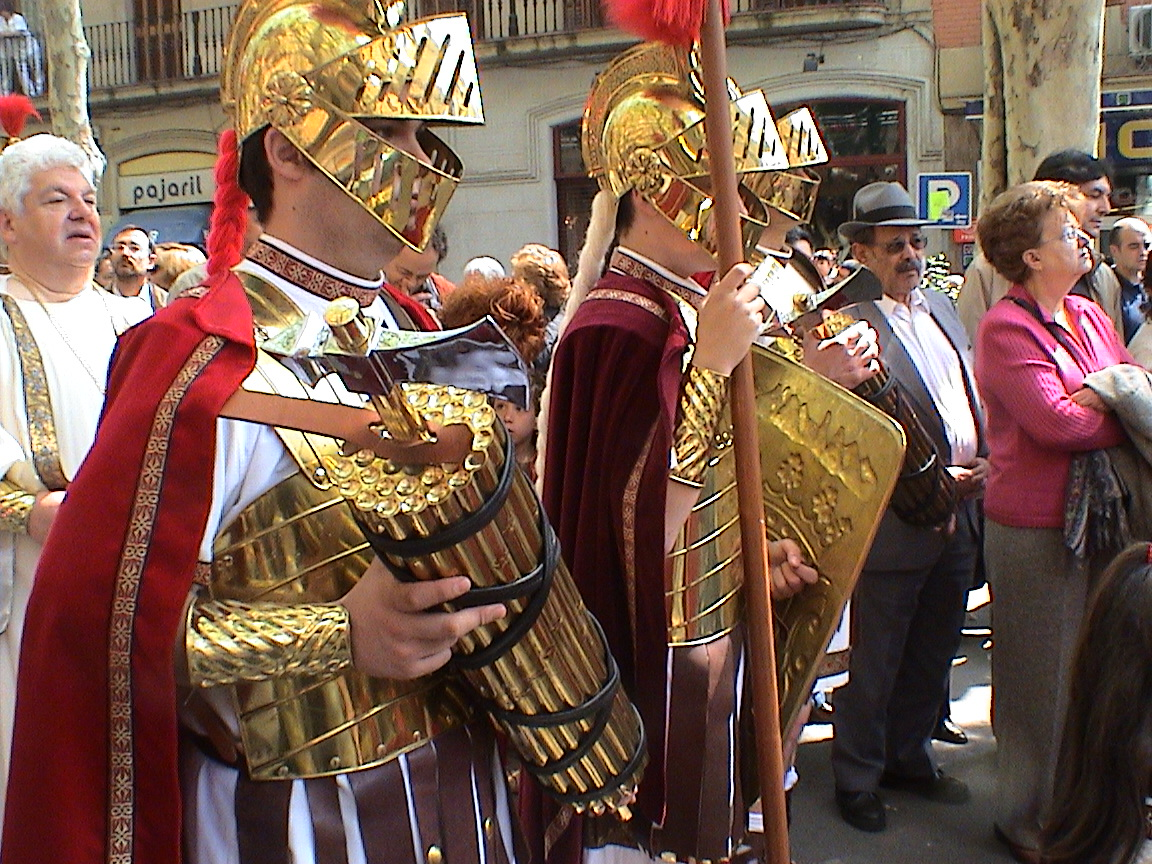
\includegraphics[width=.9\textwidth]{img/fasces/fake-fasces.jpg} \\
    Catalonia (largely autonomous Spanish province), 2006 \\
\end{frame}
\begin{frame}
    \centering
    
\includegraphics[height=.8\textheight]{img/fasces/fasces13.jpg} \\
    Adopted 1877. Text reads ``Union and Consitution''. Colorado's state website claims ``The Roman fasces is the insignia of a republican form of government\ldots The axe symbolizes authority and leadership.'' \\
\end{frame}
\begin{frame}
    \centering
    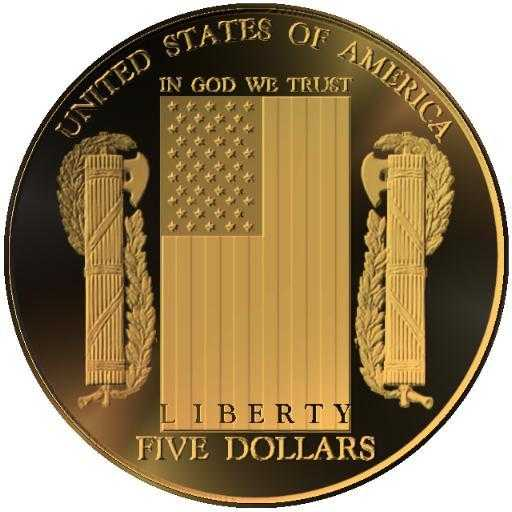
\includegraphics[height=.8\textheight]{img/fasces/fasces5coin.jpg} \\
\end{frame}
\begin{frame}
    \centering
    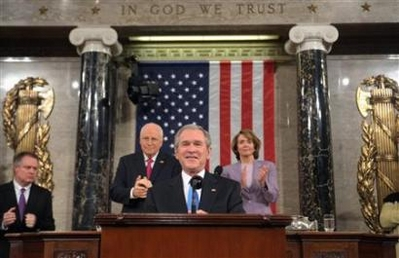
\includegraphics[width=.9\textwidth]{img/fasces/fasces_congress.jpg} \\
\end{frame}
\begin{frame}
    \centering
    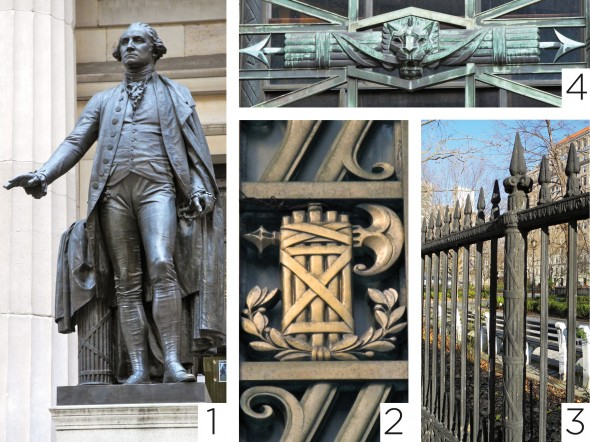
\includegraphics[width=.9\textwidth]{img/fasces/fasces-stuff.jpg} \\
    Statue by John Quincy Adams Ward, 1882.
\end{frame}
\begin{frame}
    \centering
    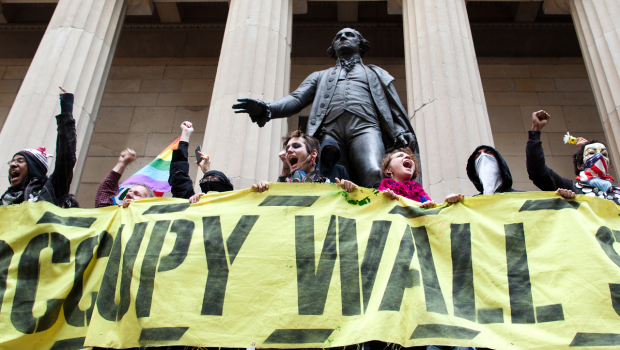
\includegraphics[width=.9\textwidth]{img/fasces/ows.jpg} \\
    Federal Hall, New York City \\
\end{frame}
\begin{frame}
    \centering
    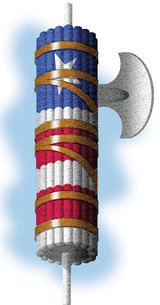
\includegraphics[height=.8\textheight]{img/fasces/flag-fasces.jpg} \\
\end{frame}
\begin{frame}
    \centering
    
\includegraphics[height=.8\textheight]{img/fasces/french-republic-symbol.png} \\
    National Symbol of France, adopted 1953. This symbol is used to represent France in the U.N. Assembly building. \\
\end{frame}
\begin{frame}
    \centering
    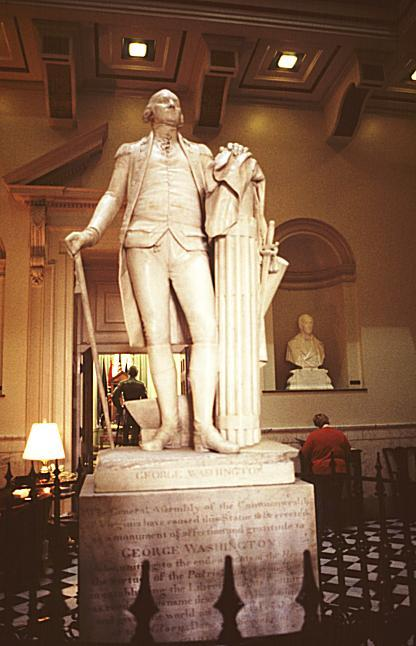
\includegraphics[height=.8\textheight]{img/fasces/houdon-front.jpg} \\
    Statue by Jean-Antoine Houdon, completed 1791. Commissioned by Virgina's legislature, and on display at Colonial Williamsburg. \\
\end{frame}
\begin{frame}
    \centering
    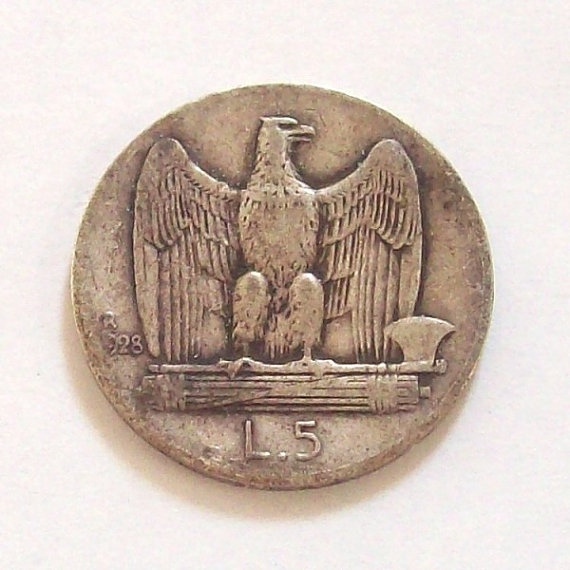
\includegraphics[height=.8\textheight]{img/fasces/italy-fasces-coin.jpg} \\
    Italian 5 lira piece, 1928 \\
\end{frame}
\begin{frame}
    \centering
    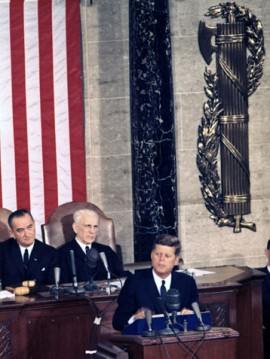
\includegraphics[height=.9\textheight]{img/fasces/jfk.jpg} \\
\end{frame}
\begin{frame}
    \centering
    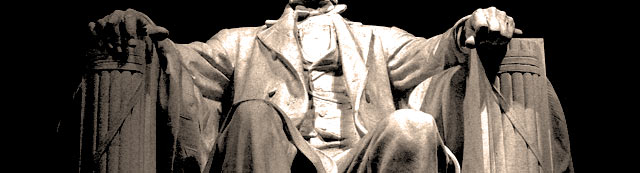
\includegraphics[width=.9\textwidth]{img/fasces/lincoln_fasces.jpg} \\
\end{frame}
\begin{frame}
    \centering
    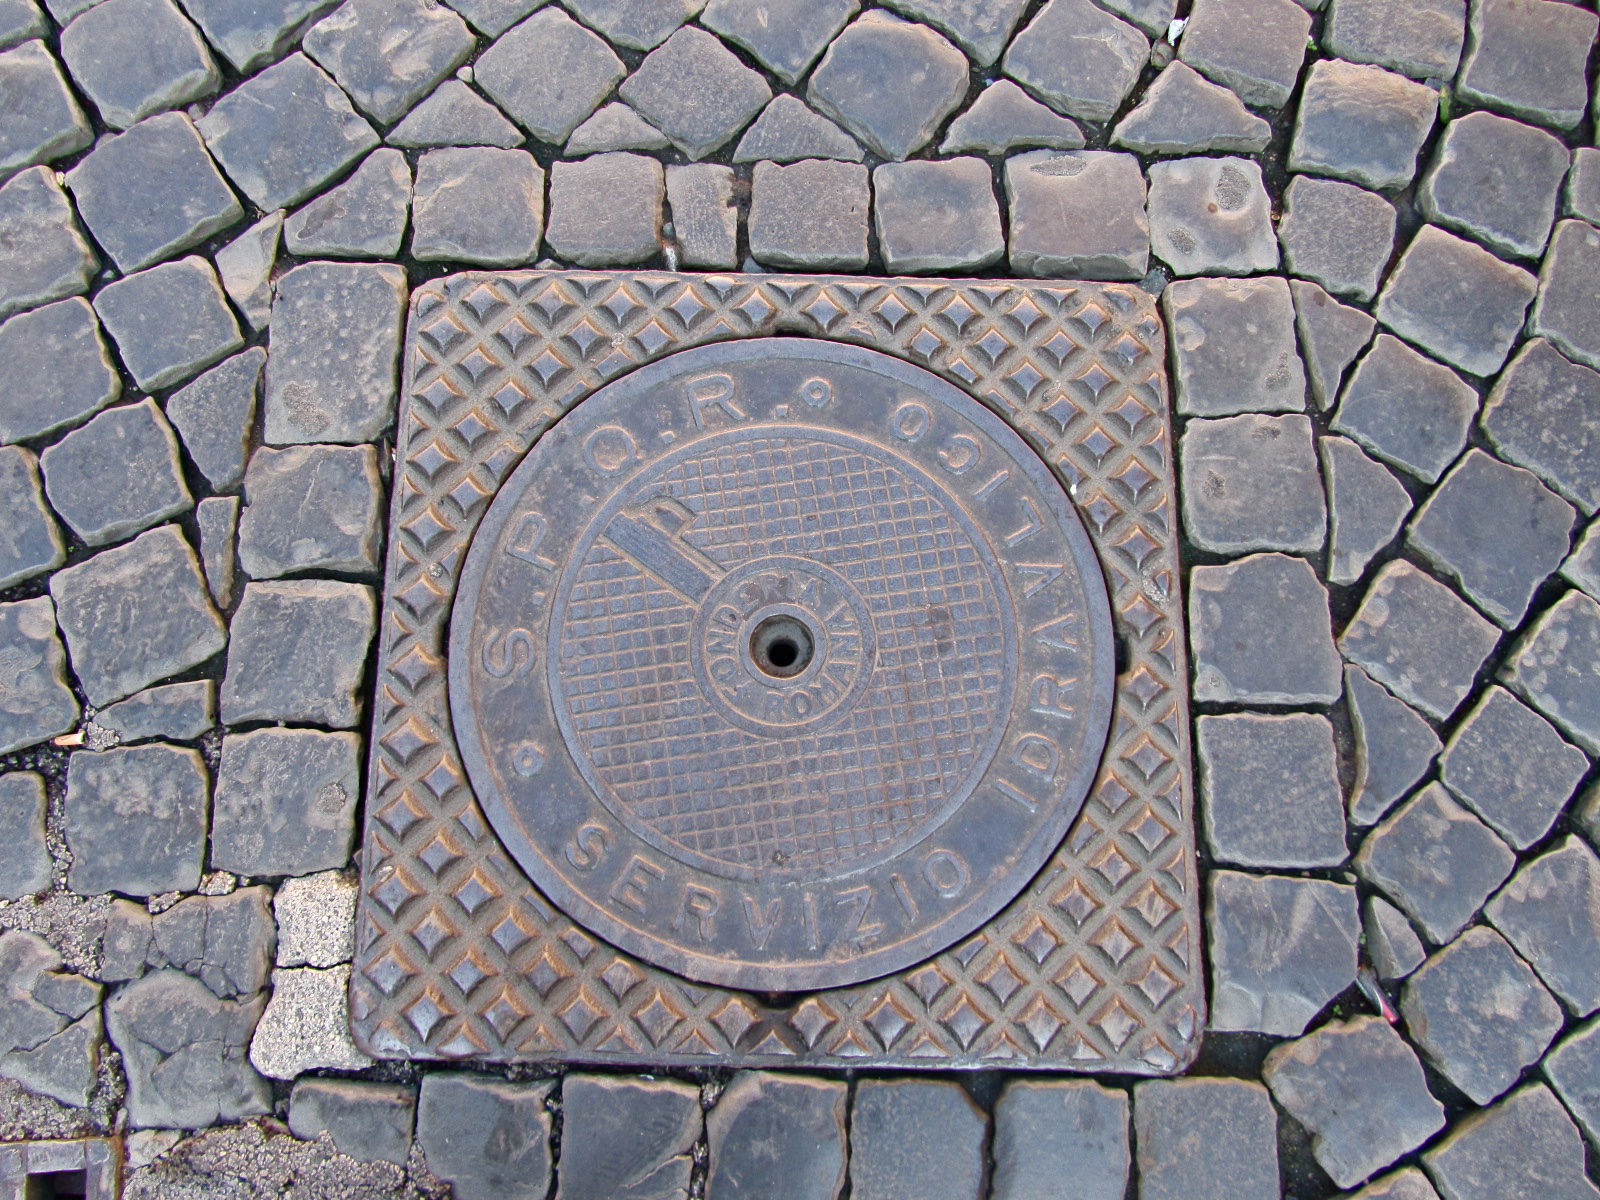
\includegraphics[width=.9\textwidth]{img/fasces/manhole.JPG} \\
\end{frame}
\begin{frame}
    \centering
    
\includegraphics[height=.8\textheight]{img/fasces/mp.jpg} \\
\end{frame}
\begin{frame}
    \centering
    
\includegraphics[height=.8\textheight]{img/fasces/tax-court.png} \\
    The Tax Court took on its present form in 1969 \\
\end{frame}
\begin{frame}
    \centering
    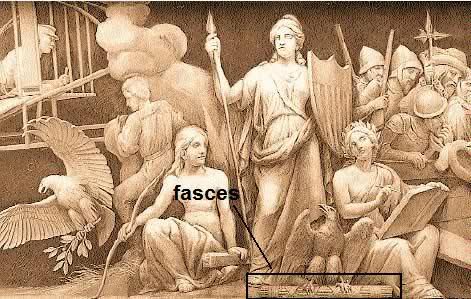
\includegraphics[height=.8\textheight]{img/fasces/teut1.jpg} \\
    Detail of frieze in the U.S. Capitol rotunda. The frieze was designed in 1859 and begun in 1877, but wasn't fully complete until 1953. \\
\end{frame}
\begin{frame}
    \centering
    \includegraphics[width=.9\textwidth]{img/fasces/tunnel.jpg} \\
\end{frame}
\begin{frame}
    \centering
    \includegraphics[height=.8\textheight]{img/fasces/washington1.jpg} \\
    By Horatio Greenough, completed in 1840, and now found in the Smithsonian
    museum of American History. The base reads,``Horatio Greenough made this
    image as a great example of freedom, and will not survive without freedom
    itself.''
\end{frame}

\begin{frame}
    \centering
    \includegraphics[width=.9\textwidth]{img/reich-stamp.png} \\
\end{frame}

\begin{frame}{Two Contending Forces}
    \begin{columns}[onlytextwidth]
        \column{0.5\textwidth}
            \begin{varblock}[0.9\textwidth]{}\huge{ \centering Sovereignty of the National Government \\}\end{varblock}

        \column{0.5\textwidth}
            \begin{varblock}[0.9\textwidth]{}\huge{ \centering Sovereignty of the individual States \\}\end{varblock}
    \end{columns}
    \textbf{\huge{ \color{red}
        \Put(155,120){v.}
    }}
\end{frame}

\begin{frame}
    \centering
    \includegraphics[width=.9\textwidth]{img/supremecourtfasces.jpg} \\
    \large{ Front of the Supreme Court building } \\
\end{frame}

\begin{frame}
    \centering
    \includegraphics[height=.85\textheight]{img/fasces_west_supcourt.jpg} \\
    \large{ On November 28, 2008, 172 pounds of this facade fell four stories to land on the steps of the court } \\
\end{frame}

\begin{frame}
    \centering
    \includegraphics[height=.9\textheight]{img/moses_east_supcourt.jpg} \\
    \large{ Rear of the Supreme Court building } \\
\end{frame}

\begin{frame}
    \centering
    \includegraphics[width=.9\textwidth]{img/10-commandments.jpg} \\
\end{frame}

\section{Empire of Debt}
\begin{frame}
    \centering
    \large{ Section 2: Empire of Debt } \\
\end{frame}

\myquote{Dr. Ron Paul}{img/ron-paul-quotepage.png}{``Demand honesty in money!''}
\myquote{Dr. Ron Paul, 15 Feb 2006}{img/ron-paul-quotepage.png}{``In earlier times it was accepted that fair and honest trade required an exchange for something of real value.''}

\begin{frame}{Silver Denarius of Julius Caesar, 44 B.C.}
    \centering
    \includegraphics[width=0.8\textwidth]{img/denarius.png} \\
    \only<2>{%
    \begin{textblock}{70}[0,1](5,96)
        \begin{varblock}[0.9\paperwidth]{}%[shadow=false,rounded=true]{box2}
        %\colorbox{SeaGreen}{%
        %    \begin{minipage}[b]{0.95\paperwidth}
                %\pgfsetfillopacity{0.35}
                \begin{centering}
    The typical Roman soldier earned 225 denarii annually \\
                \end{centering}
        %    \end{minipage}
        %}
        \end{varblock}
    \end{textblock}
    }
\end{frame}

\begin{frame}{Coin Clipping}
    \centering
    \includegraphics[height=0.6\textwidth]{img/denarius-clipping.png} \\
\end{frame}

{    \usebackgroundtemplate{%
      \vbox to \paperheight{\vfil\hbox to \paperwidth{\hfil\includegraphics[height=\paperheight]{img/denarius-bkgnd.png}\hfil}\vfil}
    }
\begin{frame}{Debasing the Denarius}
    \begin{itemize}
        \item In 54 A.D., the denarius was 94\% silver
        \item In 218 A.D., it was 43\% silver
        \item In 100 A.D., a bushel of wheat cost 3 denarii
        \item In 344 A.D., a bushel of wheat cost 2 million denarii
    \end{itemize}
\end{frame}
}

{
    \usebackgroundtemplate{%
      \vbox to \paperheight{\vfil\hbox to \paperwidth{\hfil\includegraphics[height=\paperheight]{img/silver-half-dollar-bkgnd.png}\hfil}\vfil}
    }
% XXX Add img/silver-half-dollar.png to the background, and a denarius to the background of the last "debasing" slides
\begin{frame}{Debasing the American ``silver'' half-dollar}
    \begin{itemize}
        \item In 1964, it was 90\% silver
        \item In 1969, it was 40\% silver
        \item Today, it is not silver at all
    \end{itemize}
    \vspace{63pt}
    \begin{minipage}[b]{\textwidth}
    \hfill \small{Penny Candy, p. 26}
    \end{minipage}
\end{frame}
}

\begin{frame}{A Lesson from the Khan Family}
    \begin{columns}[onlytextwidth]
        \column{0.5\textwidth}
            \centering
            \includegraphics[height=0.75\textheight]{img/khan.jpg} \\
            Kublai Khan, 1270 A.D.

        \column{0.5\textwidth}
        \begin{textblock}{60}[0,0](40,30)
            \begin{varblock}[0.9\textwidth]{}%[shadow=false,rounded=true]{box2}
            After adding greatly to the Mongol empire, Kublai Khan issued
            massive quantities of fiat currency made from mulberry tree bark.
            This worked very well until inflation took hold suddenly in 1287,
            beginning a period of disorder and warfare.
            \end{varblock}
        \end{textblock}
    \end{columns}
\end{frame}

\begin{frame}{Definitions}
    \begin{columns}[onlytextwidth]
        \column{0.5\textwidth}
        \begin{textblock}{60}[0,0](4,30)
            \begin{varblock}[0.9\textwidth]{Inflation}%[shadow=false,rounded=true]{box2}
                An increase in the amount of money
            \end{varblock}
        \end{textblock}

        \column{0.5\textwidth}
            \centering
            \includegraphics[height=0.75\textheight]{img/einstein.png} \\

    \end{columns}
\end{frame}

\begin{frame}{Definitions}
    \begin{columns}[onlytextwidth]
        \column{0.5\textwidth}
        \begin{textblock}{60}[0,0](4,30)
            \begin{varblock}[0.9\textwidth]{Fiat currency}%[shadow=false,rounded=true]{box2}
                Paper money made legal tender by decree, such as Federal Reserve Notes.
            \end{varblock}
        \end{textblock}

        \column{0.5\textwidth}
            \centering
            \includegraphics[height=0.75\textheight]{img/einstein.png} \\

    \end{columns}
\end{frame}

\myquote{Ron Paul, Chairman, House Domestic Monetary Policy Sub-Committee}{img/ron-paul-quotepage.png}{%
    ``Historically legal tender laws have been used by governments to force their citizens to accept debased and devalued currency.''%
}

\myquote{Lincoln as a young lawyer, 1838}{img/young-lincoln.jpg}{``If destruction be our lot, we must our-selves be its author and finisher.  As a nation of freemen, we must live through all time, or die by suicide.''}
\myquote{John Denson, ``A Century of War'', 2006}{img/john-denson.jpg}{``Abraham Lincoln himself became the principal instigator of America's suicide.  It was not a foreign foe, but it was a war, even a `victorious' war, that ended the Founder's dream in America.  However, leftist intellectuals have never revealed to the American people the real cause and effect of the Civil War, and instead proclaim it a `noble war' to free the slaves and therefore worth all the cost\ldots''}
\myquote{John Denson, ``A Century of War'', 2006}{img/john-denson.jpg}{``Lincoln had acted initially and primarily only to secure the economic and political domination of the North over the South.  At the end of the war he finally seemed to understand the real costs as revealed by this statement:''}
\myquote{Lincoln, after the War Between the States}{img/old-lincoln.jpg}{``As a result of the war, corporations have been enthroned and an era of corruption in high places will follow, and the money power of the country will endeavor to prolong its reign by working upon the prejudices of the people until wealth is aggregated into the hands of a few and the Republic is destroyed.''}
\myquote{Salmon P. Chase, Treasury Secretary, 1861-1864}{img/salmon-chase.png}{``My agency in promoting the passage of the National Bank Act [of 1863] was the greatest financial mistake of my life.  It should be repealed.''}
\myquote{Ben Bernanke, Nov. 21, 2002}{img/bernanke.png}{``The U. S. government has a technology, called a printing press  (or, today, its electronic equivalent), that allows it to produce as many U.S. dollars as it wishes at essentially no cost.''}

\begin{frame}
    \centering
    \includegraphics[height=\textheight]{img/notes-highlight.png} \\
\end{frame}

\begin{frame}
    \centering
    \includegraphics[width=\textwidth]{img/silly-fed-picture.png} \\
\end{frame}

\myquote{John Adams}{img/john-adams.jpg}{``Every dollar of a bank bill that is issued beyond the quantity of gold and silver in the vaults represents nothing, and is therefore a cheat upon somebody.''}

\myquote{British economist John Maynard Keynes, 1944}{img/keynes.jpg}{``National debt doesn’t really matter, we just owe it to ourselves.''}
\myquote{British economist John Maynard Keynes, 1944}{img/keynes.jpg}{``We should spend ourselves into prosperity.''}

\myquote{Isaiah 5:13; Image of ``Christ the King'' statue, in Świebodzin, Poland}{img/christ-statue.jpg}{``Therefore my people are gone into captivity, because they have no knowledge: and their honourable men are famished, and their multitude dried up with thirst.''}

\end{document}
